\subsection{CRUD}

As mentioned, the main focus of this sprint was to get the server up and running for the other layers. 
As we already had a working database, the goal of this increment was to write a CRUD API in C\# such that the other layers could use to access the database via HTTP requests.
The CRUD operations we implemented are based on requests from the other layers, and what they thought they needed to retrieve from the database.
% To use data sent to us from the other layers we had to imlement a JSONModel  for each table they needed to insert data into.
% DB model and JSONModel
    % why use DB model and JSON model?
To implement this, we split the CRUD operations into three different APIs handling different aspects of the database. Each API is is accessing different tables in the database.
% hvorfor har vi forskellige APIer?
The pipeline for these APIs is outlined in figure \ref{Node02Sprint3}.

\begin{figure}[h]
    \centering
    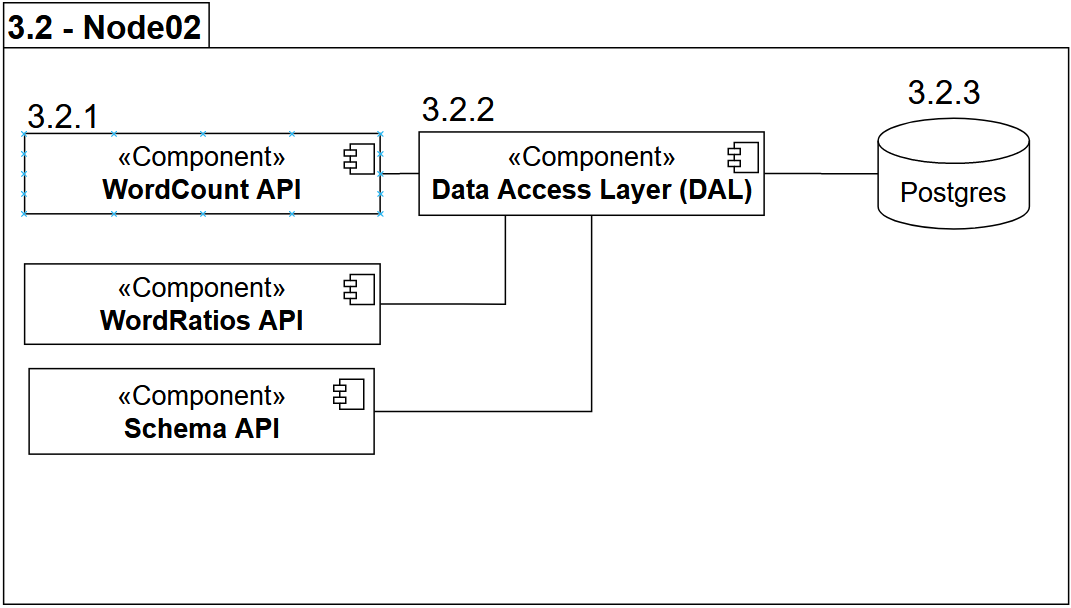
\includegraphics[width=\linewidth]{Images/Node02Sprint3.PNG}
    \caption{Node02 server pipeline in sprint 3.}
    \label{Node02Sprint3}
\end{figure}

\subsubsection{WordCount API}

The first API we created was the WordCount API. It is used by the knowledge layer to insert information about an article into the database. It is also used by the functionality layer to find the filepath of an article.

In the API we implemented 2 methods, a \texttt{GET} and a \texttt{POST} method.
\begin{table}[h]
    \begin{tabular}{|llll|}
    \hline
    \multicolumn{4}{|c|}{\textbf{WordCount API}}                                                                                 \\ \hline
    \multicolumn{1}{|l|}{Name}                 & \multicolumn{1}{l|}{Method} & \multicolumn{1}{l|}{Input}       & Response on success       \\ \hline
    \multicolumn{1}{|l|}{\texttt{GetFilepath}} & \multicolumn{1}{l|}{GET}    & \multicolumn{1}{l|}{Integer}     & Article        \\ \hline
    \multicolumn{1}{|l|}{\texttt{Post}}        & \multicolumn{1}{l|}{POST}   & \multicolumn{1}{l|}{JSON Object} & Status message \\ \hline
    \end{tabular}
    \end{table}

The \texttt{GET} method called \texttt{GetFilepath}, takes a integer "id" as an argument and finds an article in the database with the given "id" and returns the articles filePath as a JsonResult if it exists, otherwise an error is sent back.


In the WordCount API, we also implemented a \texttt{POST} method called \texttt{Post} which takes a JSON object from the HTTP body as a parameter. 
The JSON object should be valid according to a JSONschema on the database, which determines the required format of the of the JSON object and the fields needed. If the JSON object does not fit the schema, an error message is sent back. 
The input is then checked for duplicate data on the database, if there is any it is removed and a message is added to the response that the article already exists. The remaining articles can then be inserted into the database, and a status message is returned with the potential duplicate article names. 
 
\subsubsection{WordRatios API}
The WordRatios API is used by the functionality layer to fetch specific data from the database.
As the WordRatio table is a view, it cannot be used to store new data. 
The primary purpose of the WordRatios API is to check how many times a given word occours in an article.
The API consists of one \texttt{GET} method with an optional parameter. 
\begin{table}[h]
    \begin{tabular}{|llll|}
    \hline
    \multicolumn{4}{|c|}{\textbf{WordRatios API}}                                                                                                                                           \\ \hline
    \multicolumn{1}{|l|}{Name}                      & \multicolumn{1}{l|}{Method} & \multicolumn{1}{l|}{Input}                           & Reponse on success                               \\ \hline
    \multicolumn{1}{|l|}{\texttt{GetMatches}}       & \multicolumn{1}{l|}{GET}    & \multicolumn{1}{l|}{terms (string []), sources (string[])} & WordRatio for all articles from source with term \\ \hline
    \multicolumn{1}{|l|}{\texttt{GetMatches}}       & \multicolumn{1}{l|}{GET}    & \multicolumn{1}{l|}{terms (string [])}                   & WordRatio for all articles with term             \\ \hline
    \end{tabular}
    \end{table}
The \texttt{GetMatches} method is used to query one or more specific words on the WordRatio table.
One may provide one or more sources in which to search for the specified words.
If no sources are provided, the database searches for the given words in all sources.
The Rows of the table matching the terms and sources.

\subsubsection{Schema API}
The last API we implemented in this iteration is the Schema API which is used to post and retrieve a JSON schema from the database. These are later used to verify JSON objects as input on other APIs. 
This API concists of two \texttt{GET} methods and a single \texttt{POST} method.
By creating an API for fetching the validation schemas, we enable easy validation and a common understanding of the structure of input data from the knowledge layer.
\begin{table}[h]
    \begin{tabular}{|llll|}
    \hline
    \multicolumn{4}{|c|}{\textbf{Schema API}}                                                                                                     \\ \hline
    \multicolumn{1}{|l|}{Name}                     & \multicolumn{1}{l|}{Method} & \multicolumn{1}{l|}{Input}               & Response on success \\ \hline
    \multicolumn{1}{|l|}{\texttt{GetSchema}}       & \multicolumn{1}{l|}{GET}    & \multicolumn{1}{l|}{SchemaName (string)} & JSON Schema         \\ \hline
    \multicolumn{1}{|l|}{\texttt{GetAllSchemas}}   & \multicolumn{1}{l|}{GET}    & \multicolumn{1}{l|}{None}                & All JSON Schemas    \\ \hline
    \multicolumn{1}{|l|}{\texttt{PostJSONSchemas}} & \multicolumn{1}{l|}{POST}   & \multicolumn{1}{l|}{JSON Schema}         & Status message      \\ \hline
    \end{tabular}
    \end{table}

The first \texttt{GET} method is called GetSchema which takes a SchemaName as its input and returns a JSON Schema. 

The second \texttt{GET} method is called GetAllSchemas which takes no input and returns all stored JSON schemas. 

The last method is a \texttt{POST} method called PostJSONSchema and takes a JSON Schema as its input and inserts it into the database.
The body of the post request must consist of two fields - the schema name, which is its primary key in the database, and the schema content itself. Before the schema is inserted in the database it is checked if it is a duplicate, if that is the case an error message will be sent in response.
A schema gets stored in the database in the format known as \texttt{jsonb} or JSON binary which is a built-in type provided by \postgres{}.
This format is used to store a JSON object as binary which uses much less space than a varchar or regular JSON type would.
Even though \postgres{} may not be the most efficient DBMS for storing JSON data, it is sufficient for this usecase, as posting and fetching Schemas will not be done often.



\todo{Mention earlier that the database was accesed directly, instead of through an API}
\todo{Describe our models}
\todo{Describe how data is accessed with EF Core}
\todo{Describe the structure of the database}

